\chapter{SpinTaylorF2 waveform -- Overlap Study} 

\label{chap:SpinTaylorF2} 
\section{Construction of SpinTaylorF2} 

The SpinTaylorF2 waveform~\cite{Lundgren2014} is a single spin, frequency domain
waveform that incorporates the effects of precession.  The waveform model
assumes one component of the binary to have negligible or zero spin, and
describes the inspiral phase~\cite{Event_0} of the signal. We will therefore
restrict our attention to NS-BH binaries since the neutron star in these systems
are expected to have neglible spins. Consider a NS-BH binary, with black hole
mass $m_{1}$ and dimensionless spin $\chi_{1} = |\mathbf{S}|/m_{1}^2$ where
$|\mathbf{S}|$ is the spin angular momentum of the black hole, and a neutron
star with mass $m_{2}$ and zero spin. The the symmetric mass ratio $\eta$ is
defined as $\eta=m_{1}m_{2}/M^2$. where $M$ corresponds to the total mass of the
binary $(m_{1} + m_{2})$.  Further, we can define the total angular momentum
vector $\mathbf{J}=\mathbf{L} + \mathbf{S}$ of the binary as a sum of the
orbital anuglar momentum vector $\mathbf{L}$. We also define a quantity
$\kappa=\hat{\mathbf{L}}\cdot\hat{\mathbf{S}}$, to describe the alignment of the
$\mathbf{L}$ and $\mathbf{S}$: $\kappa=0$ corresponds to the situation where
$\mathbf{L}$ and $\mathbf{S}$ are perpendicular to each other, and $\kappa=\pm
1$ correponds to the aligned (anti-aligned) case. In addition, polar angles
$(\theta_{J}, \psi_{J})$  describes the relative orientation  of the total
angular momentum vector $\mathbf{J}$ with the line of sight unit vector
$\hat{\mathbf{N}}$ (see, for eg.,~\cite{thetaJ} for a graphical representation
of the coordinates used). All the equations in the report are written in 
$\left[G = c = M_{\odot }= 1\right]$ units.

If the black hole has non-zero spin, and the spin-angular momentum $\mathbf{S}$
is  not aligned with the orbital orbital angular momentum $\mathbf{L}$ of the
binary, the plane of orbital motion inclines and precesses over
time~\cite{Apostolatos1994}: both $\mathbf{L}$ and $\mathbf{S}$  would precess
about the total angular momentum vector $\mathbf{J}$ (see Eq.~(11)
in~\cite{Apostolatos1994} for evolution equations of $\mathbf{L}$ and
$\mathbf{S}$). Further, if $\mathbf{L}$ and $\mathbf{S}$ do not cancel each
other (i.e. are not antialigned and almost equal in magnitude)  the binary
undergoes simple precession~\cite{Apostolatos1994}, where $\mathbf{J}$ remains
nearly fixed during the inspiral, and $\mathbf{L}$ and $\mathbf{S}$ precesses
about $\mathbf{J}$ with a uniform angular velocity. The SpinTaylorF2 waveform
assumes simple precession~\cite{Lundgren2014}, and breaks down  when the
assumption is no longer applicable.

\label{fig:waveforms} 
\begin{figure}[t]
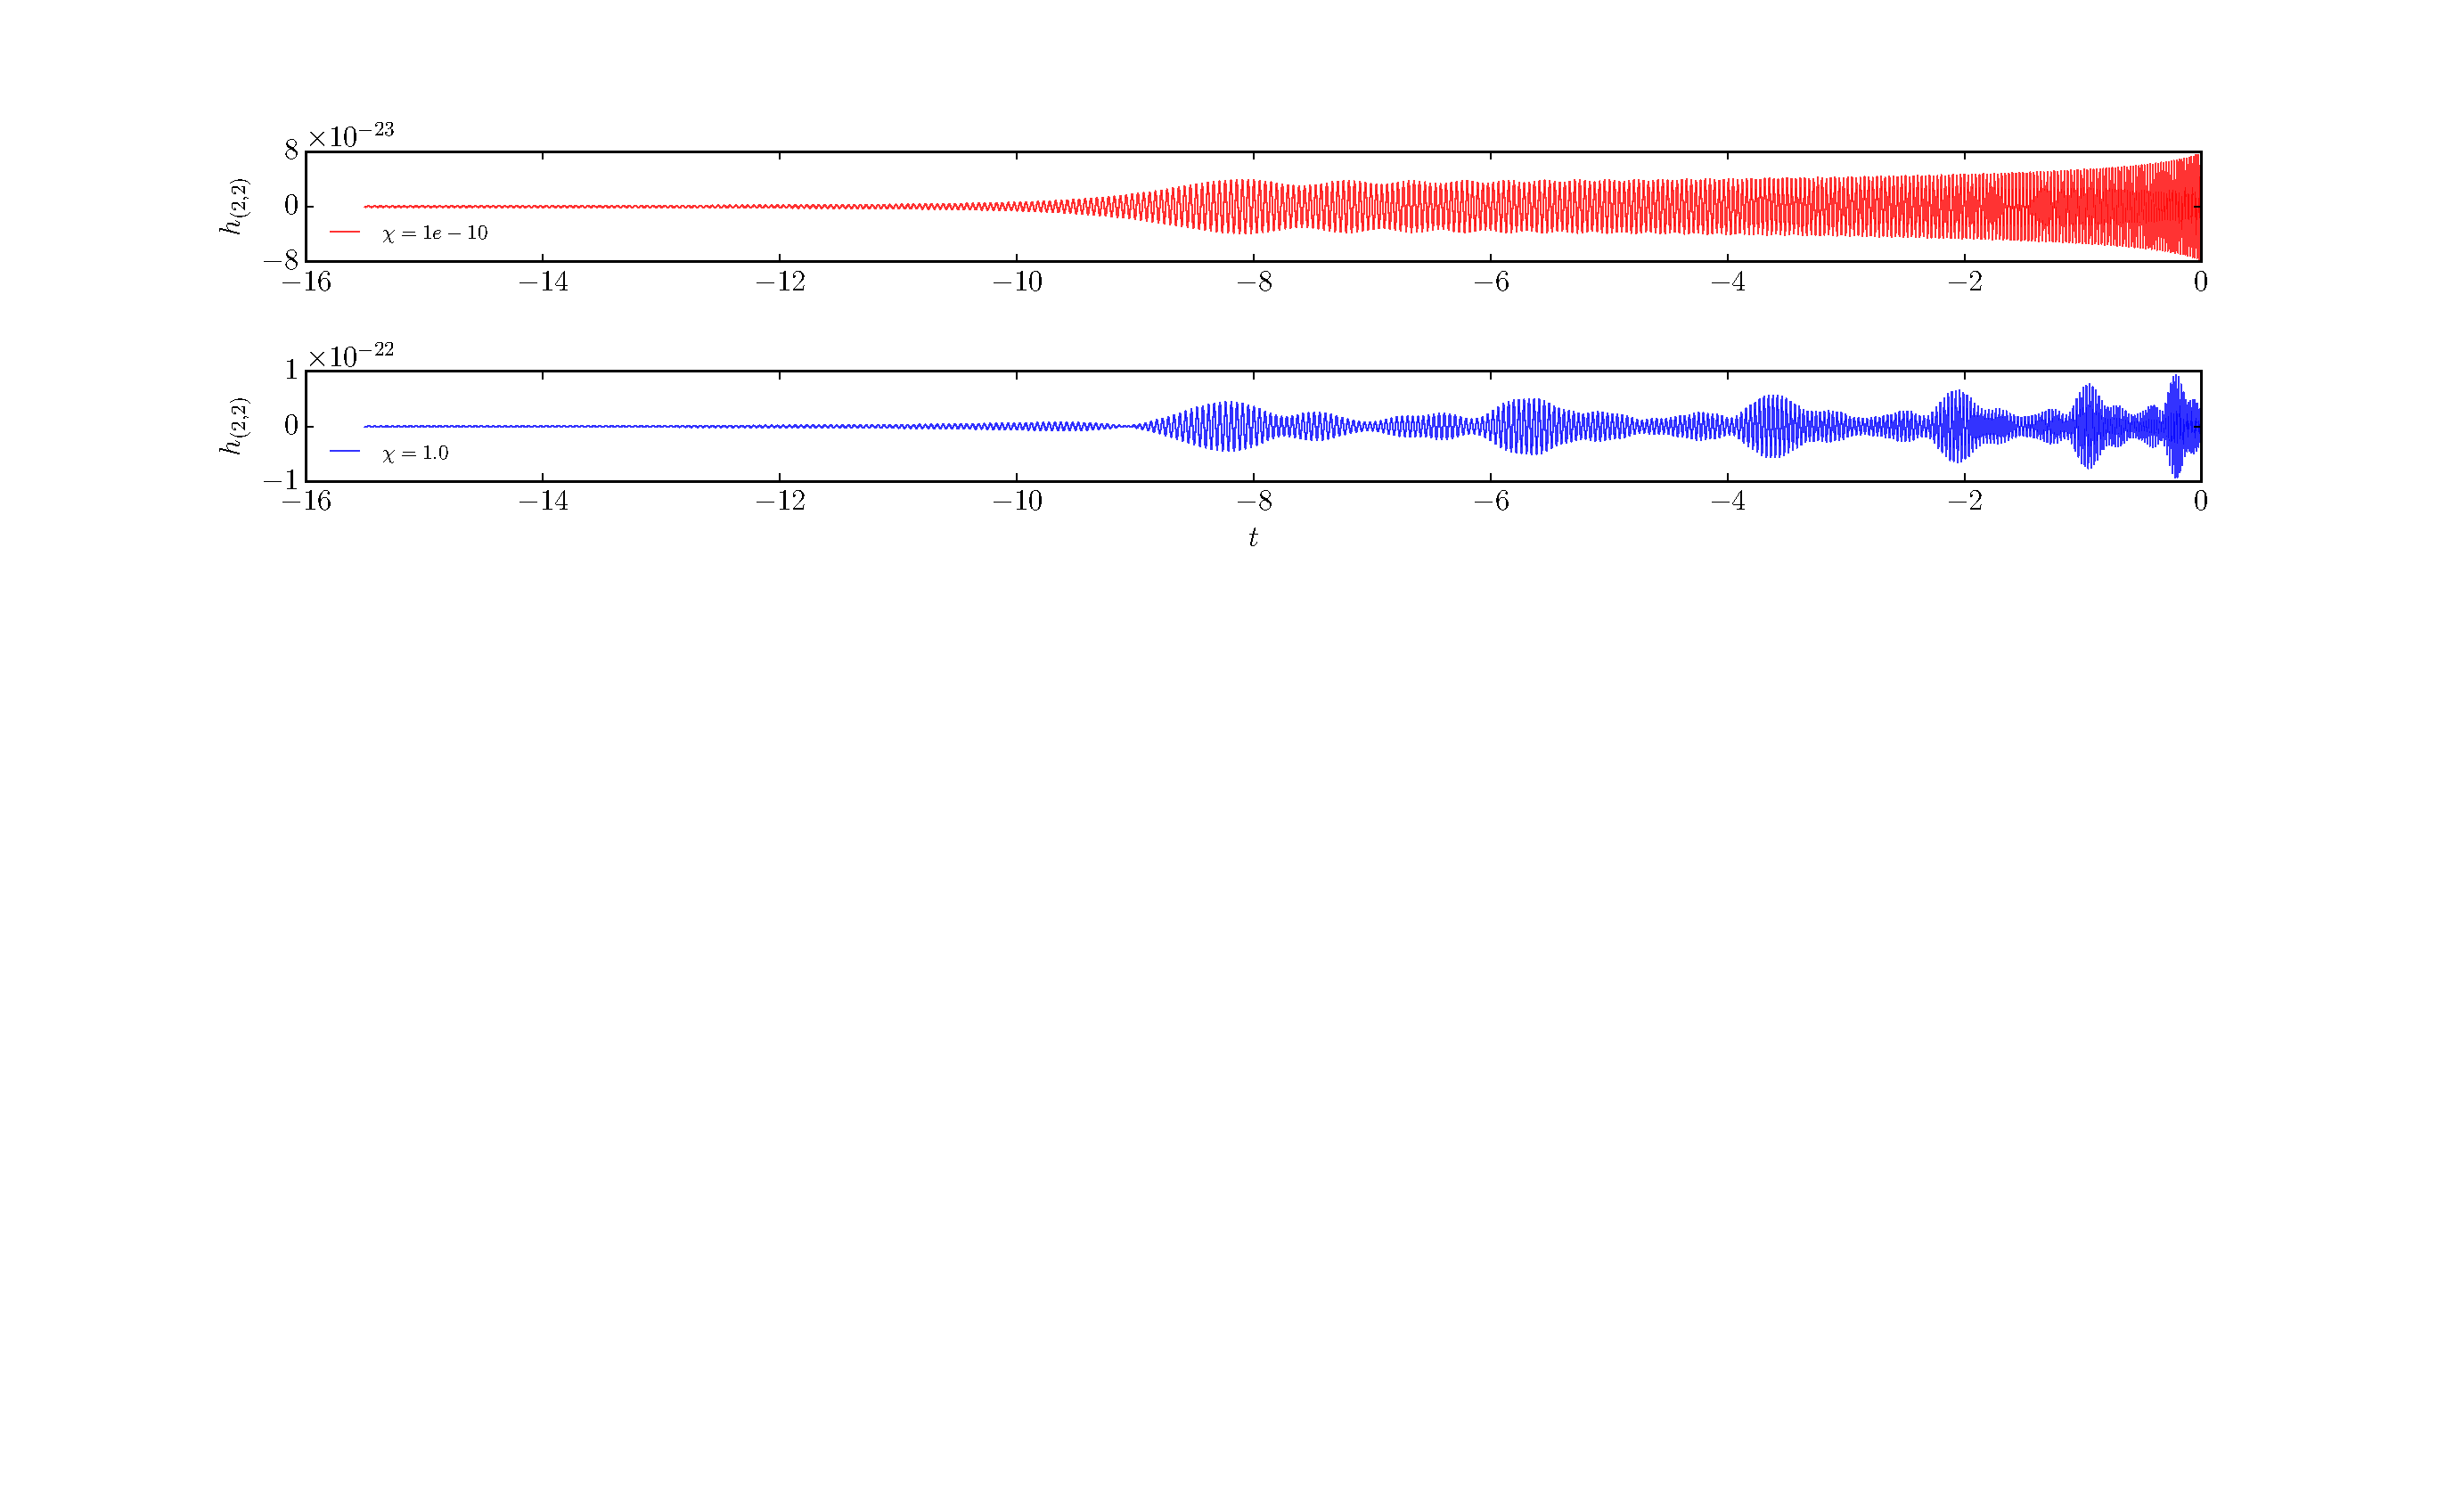
\includegraphics[width=\textwidth]{./images/TD_waveforms_comparison.pdf}
\caption{SpinTaylorF2 waveforms for non-precessing (red) and precessing (blue) system. 
The modulations in the waveform amplitude due to precession is clearly visible in the 
bottom figure.} 
\centering 
\end{figure}

The precession of the orbital plane leads to modulations in the gravitational
wave amplitude and phase in the observer's frame of reference (see Fig.~\ref{fig:waveforms}).
However, the precessing waveform in the observer's frame can be decomposed into
non-precessing waveform acted upon by a time-dependent rotation~\cite{Boyle2011,
Rotation}. The time-dependent rotation relates the observer's frame of reference
aligned with $\mathbf{J}$ to a frame that co-rotates with the precession of the
orbital angular momentum vector $\mathbf{L}$. The precessing waveform can then
be expressed as a weighted sum of the co-rotating frame amplitudes
$\tilde{h}^{l,m}$ (see Eq. (3) in~\cite{Lundgren2014}):

\begin{equation}   
h_{+} + i h_{\times} = e^{-2 \psi}
\sum_{l,m,m^{\prime}} \mathcal{D}^{l}_{m^{\prime},m} \left(\alpha, \beta, \gamma\right)
\tilde{h}^{l,m}(t){}_{-2}Y_{l,m^{\prime}}\left(\theta,\phi\right)e^{-i m \Phi},
\end{equation}   
where $\mathcal{D}^{l}_{m^{\prime},m}$ is the Wigner rotation matrix of
SU2~\cite{Boyle2011}, and $(\alpha, \beta, \gamma)$ are the time- dependent
Euler angles that relate the co-rotating frame to the observer's frame of
reference. See~\cite{Lundgren2014} for complete definitions. Considering only
the leading order $(l=2, |m| = 2)$ mode, we can express the above expression in
frequency domain using the stationary phase approximation~\cite{Lundgren2014,
Creighton}.  Upon simplification, one arrives at the following expression for
the SpinTaylorF2 waveform (see Eq. (12--13) in~\cite{Lundgren2014}):

\begin{equation}  
\label{STF2_main} 
h_{+}(f) =
\dfrac{2\pi M_{c}^{2}}{D}\sqrt{\dfrac{5}{96\pi}}(\pi M
f)^{-7/6}\sum_{m}z_{m}e^{i(\Psi - 2\zeta) + i m \alpha},
\end{equation} 
where $D$ corresponds to the distance to the source, and $M_{c}$ corresponds to
chirp mass~\cite{Creighton} of the binary. The expressions for $z_{m}, \alpha,
\Psi$ and $\zeta$  can be found in~\cite{Lundgren2014}, we omit them for
brevity. Fig.~(\ref{fig:waveforms}), shows  time-domian plot of the full
SpinTaylorF2 waveform for a precessing and non-precessing case. Each term in the
summation in Eq.~(\ref{STF2_main}) represents a single sideband that is
modulated in amplitude and phase depending on the value of $m$.  We observed
that in  the non-precessing case, only the $m=2$ sideband has a non-zero
amplitude; however, for a precessing system, all the sidebands develop a non-
zero amplitude. Thus, we would expect that the single to noise ratio (SNR) from
the total waveform would be sub-divided into the SNR contribution from each of
the individual sidebands in case of precession systems. In the following section, 
we discuss how the SNR of the total waveform is distributed among the sidebands
by computing overlap between the particular sideband and the full waveform.


\section{Computation of SNR and Overlaps}

The signal-to-noise ratio (SNR) of a frequency domain waveform $h(f)$ is given by 
$(h|h)$, where $(a|b)$ is the noise-weighted scalar product defined as 

\label{inner_product}  
\begin{equation} (a|b) = 4 \text{Re} \left[
\int_{f_{1}}^{f_{2}}  \dfrac{a^{*}(f)b(f)}{S_{n}(f)} df\right] 
\end{equation}
where $S_{n}(f)$ is the one-sided noise power spectral density (PSD) of the
detector~\cite{PSD}, and $a^{*}(f)$ is the complex conjugate of the frequency
domain waveform amplitude $a(f)$. The SNR --- as the name suggests --- indicates
how \textit{loud} the GW signal is compared to the background noise of the
detector. We compute the SNR of full SpinTaylorF2 waveform for binary systems
with  different $\chi$ and $\eta$ values, and investigate the variation of SNR
with variation in $\theta_{J}$ which specifies the orientation of the plane
binary, and $\kappa$, which indicates the the alignment of the alignment between
$\mathbf{L}$ and $\mathbf{S}$. We fix the neutron star mass $(m_{1})$ to $1.4$,
since the observations of neutron masses in BNS systems have reported a narrow
mass distribution bounded by $1.0$ to $1.4$ solar masses~\cite{Lorimer}.
Fig.~(\ref{fig:SNR}) shows the variation SNR of the SpinTaylorF2 waveform   over
$(\theta_J, \kappa)$ the parameter space, for different $\chi$ and $\eta$
values. Since we have fixed the mass of the neutron star to $1.4 M_{\odot}$, the
lower values of $\eta$ correspond to higher black hole masses.

\label{fig:SNR} 
\begin{figure}[t]
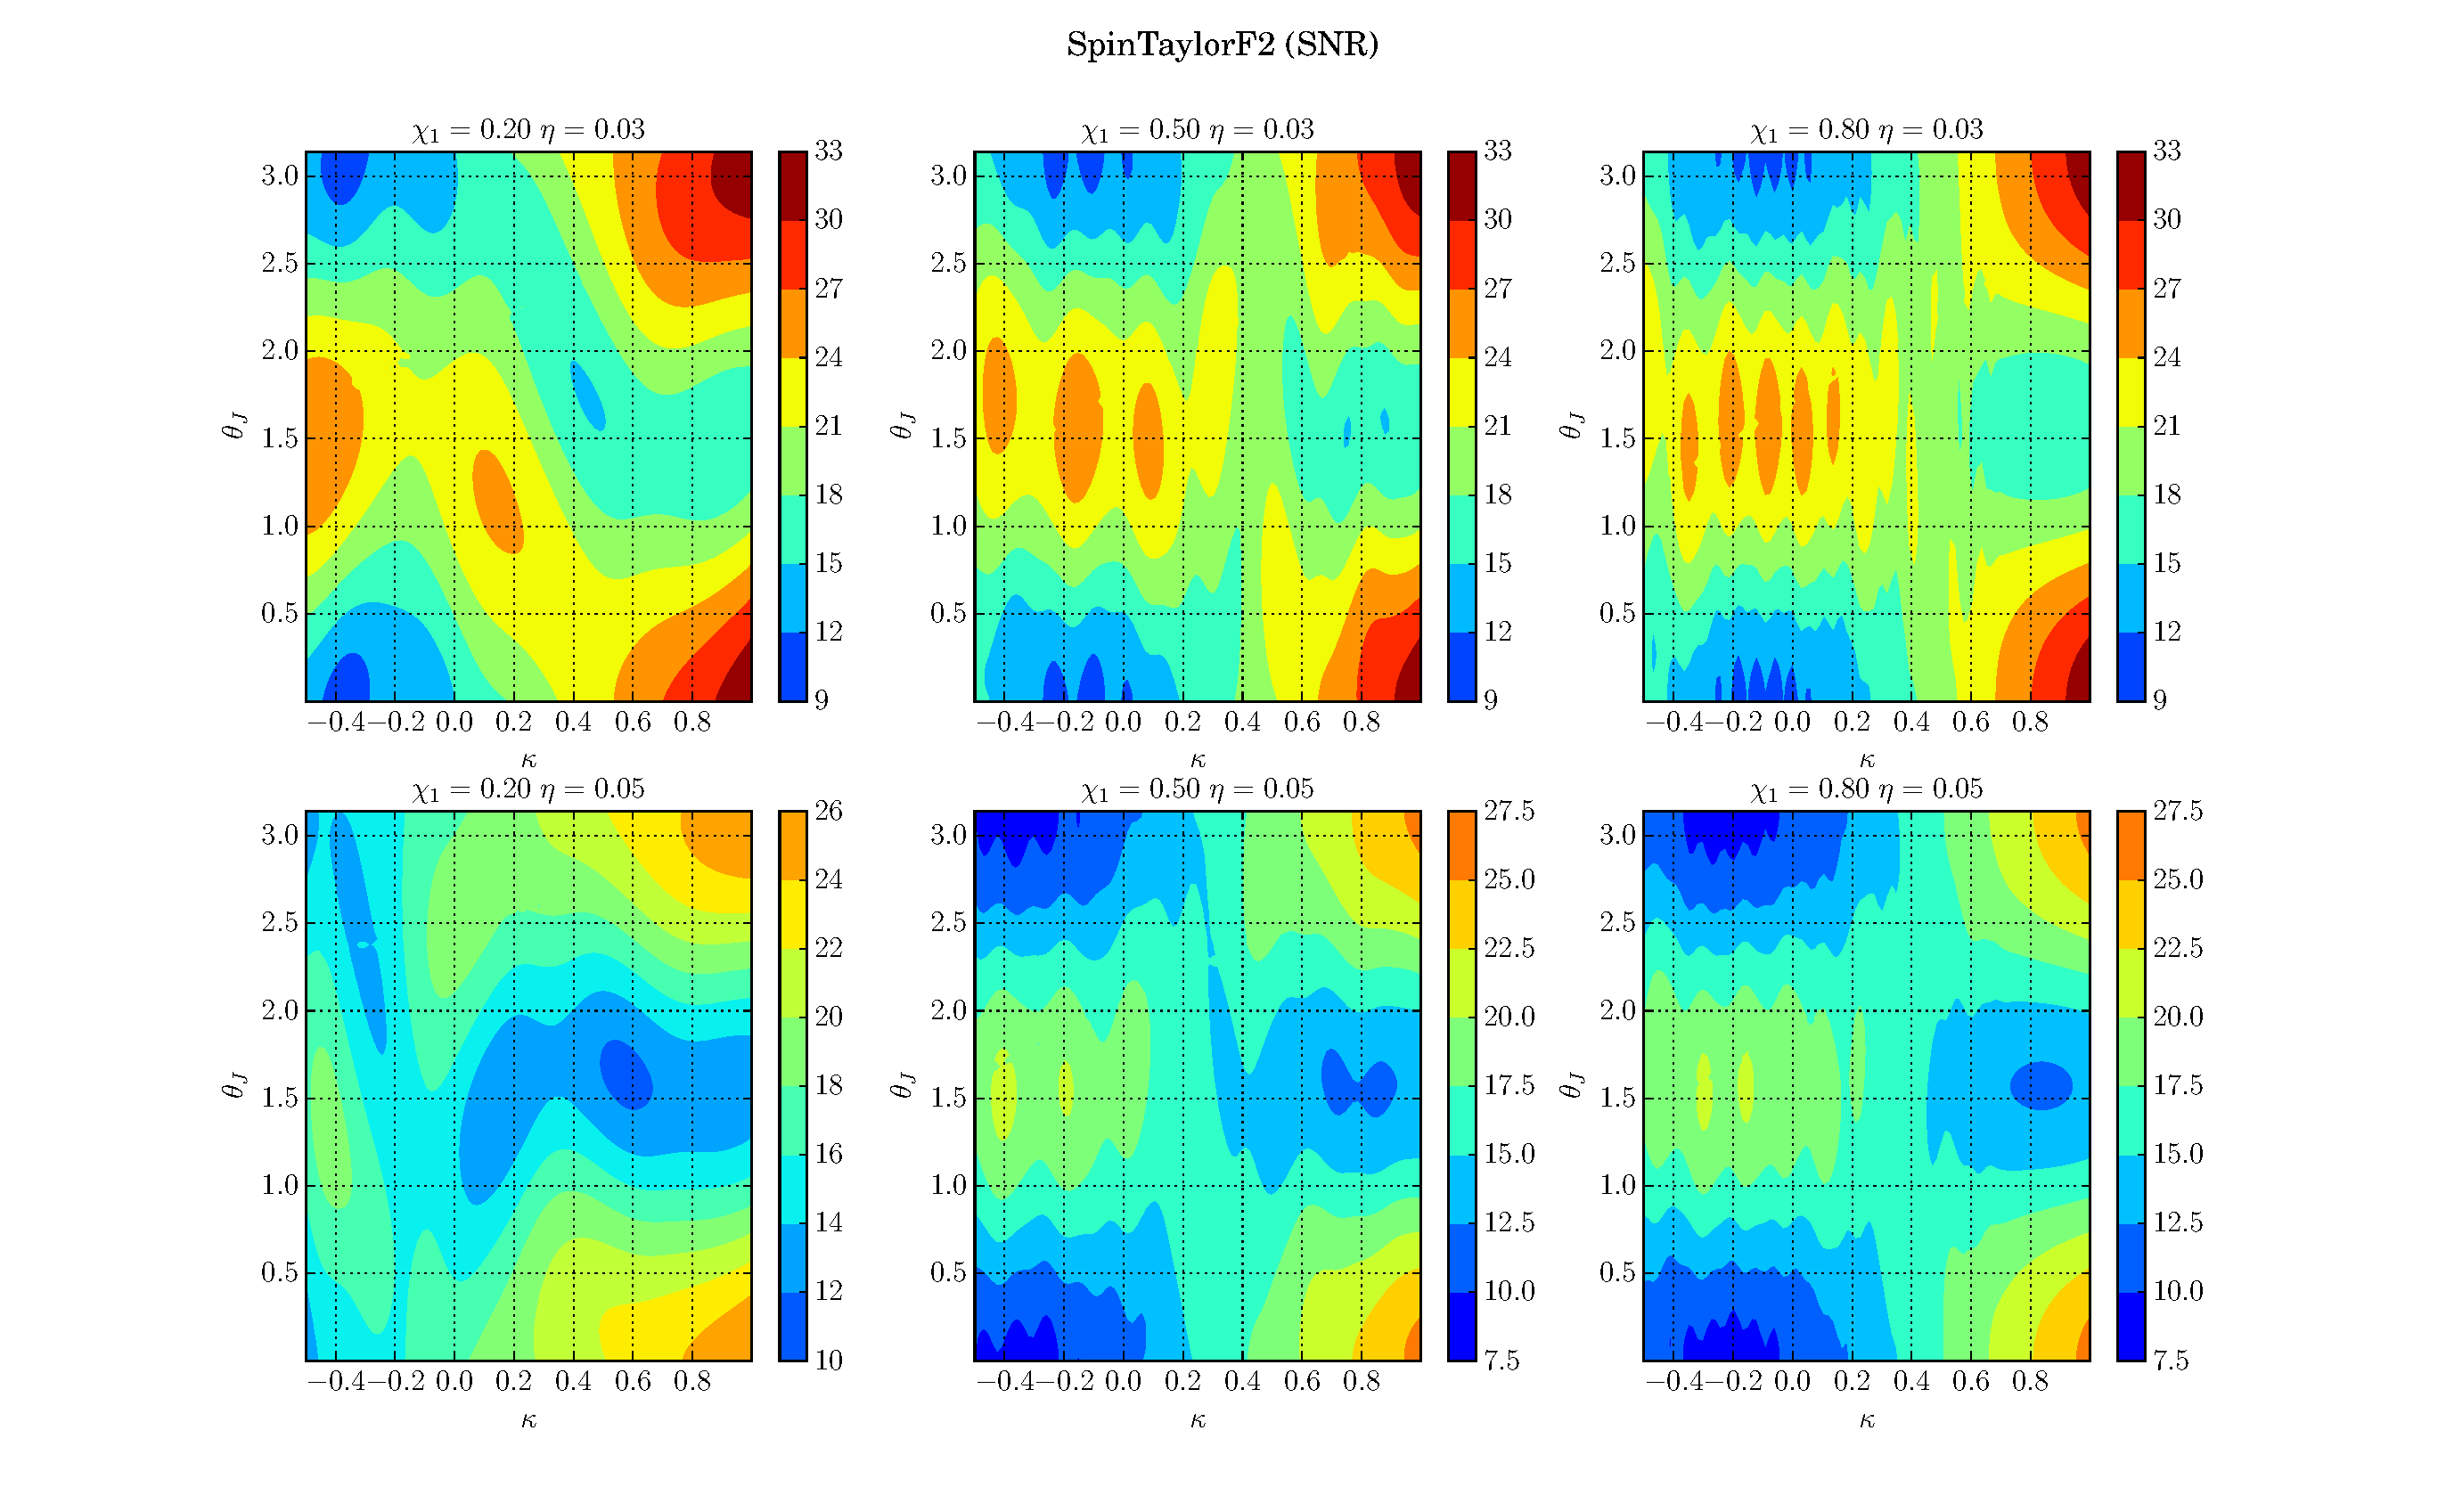
\includegraphics[width=\textwidth]{./images/SNR_GRID_0F.pdf}
\caption{Variation of SNR in the $(\theta_J, \kappa)$ parameter space for 
different $\chi$ and $\eta$ values, where $\chi$ changes over the horizontal 
axis of the grid and $\eta$ varies over the vertical axis of the grid.}
\centering 
\end{figure}

We see that the maximum SNR increases with the increase in black hole mass
(i.e. lower $\eta$). Further, we observe that the SNR is the highest in the
region where  $\theta_{J} = 0$ or $\pi$ which corresponds to the situation where
the the plane of  the binary is directly overhead or underneath us, and for
$\kappa = 1$ which means that  $\mathbf{S}$ is along the direction of
$\mathbf{L}$. Both these features can be explained by simply comparing the
results with expression for the frequency independent part of waveform amplitude 
in the presence of precession (see Eq.~(A4) in~\cite{Apostolatos1994}):
\label{amplitudes}
\begin{equation}
H_{+} = \frac{1}{2}\frac{4 m_{1}m_{2}}{rD} \left[1 + (\hat{\mathbf{L}}\cdot\hat{\mathbf{N}})^{2}\right], 
H_{\times} = \frac{4 m_{1}m_{2}}{rD}\left[\hat{\mathbf{L}}\cdot\hat{\mathbf{N}}\right].
\end{equation}
The above equation suggests that the SNR --- which is directly proportional to
the square of the  amplitude of the waveform -- increases with increasing mass,
and also the fact the amplitudes  are maximum when $\mathbf{L}$ is along the
line of sight $\hat{\mathbf{L}}$. The second condition is precisely what the
combination of $(\theta_J, \kappa)$ satisfies, in regions where the SNR peaks.
The fact that the SNR also peaks near $\theta_J = \pi/2$ for lower values of
$\kappa$, can aslo be explained using Eq.~(\ref{amplitudes}); the argument
however, is more involved.

To evaluate the fractional SNR contribution by the sidebands to the total SNR, 
we computed the overlap of each of the sidebands with the full waveform. 
The overlap between two frequency series amplitudes $a(f)$ and $b(f)$ is defined as (see~\cite{Lundgren2014}):
\begin{equation} 
O_{ab} \equiv \dfrac{(a|b)}{\sqrt{(a|a)(b|b)}},
\end{equation} 
where $(a|b)$ is the noise-weighted inner product defined in Eq.~(\ref{inner_product}).

 % We computed the
% overlaps for all the sidebands i.e. $m=-2$ to $m=2$ and found that the $m=0$ to
% $m=2$ modes are the dominant contributors to the total SNR of the full
% SpinTaylorF2 waveform. We also found that $m=0$ to $m=2$ dominate are different
% regions of the parameter space -- if the system is hihgly precessing, most of
% the SNR is captured by the $m=0$ sideband, and when the system is not precessing
% the $m=2$ has the dominant contribution to the SNR of the signal. Fig.~(3) shows
% the overlap plots for $m=2$ and $m=0$ sidebands with the full SpinTaylorF2
% waveform. This suggests that one can use the sidebands -- which are
% computationally cheaper to generate than the full SpinTaylorF2 waveform -- to
% estimate parameters in the regions where their overlap with the full
% SpinTaylorF2 waveform is very high i.e. for precessing systems one can use the
% $m=0$ for parameter estimation since the maximum contribution to the SNR is
% coming from the $m=0$ mode when the system is precessing. This would allow for a
% massive reduction in computational cost associated with waveform generation.

\label{fig:P2} 
\begin{figure}[t]
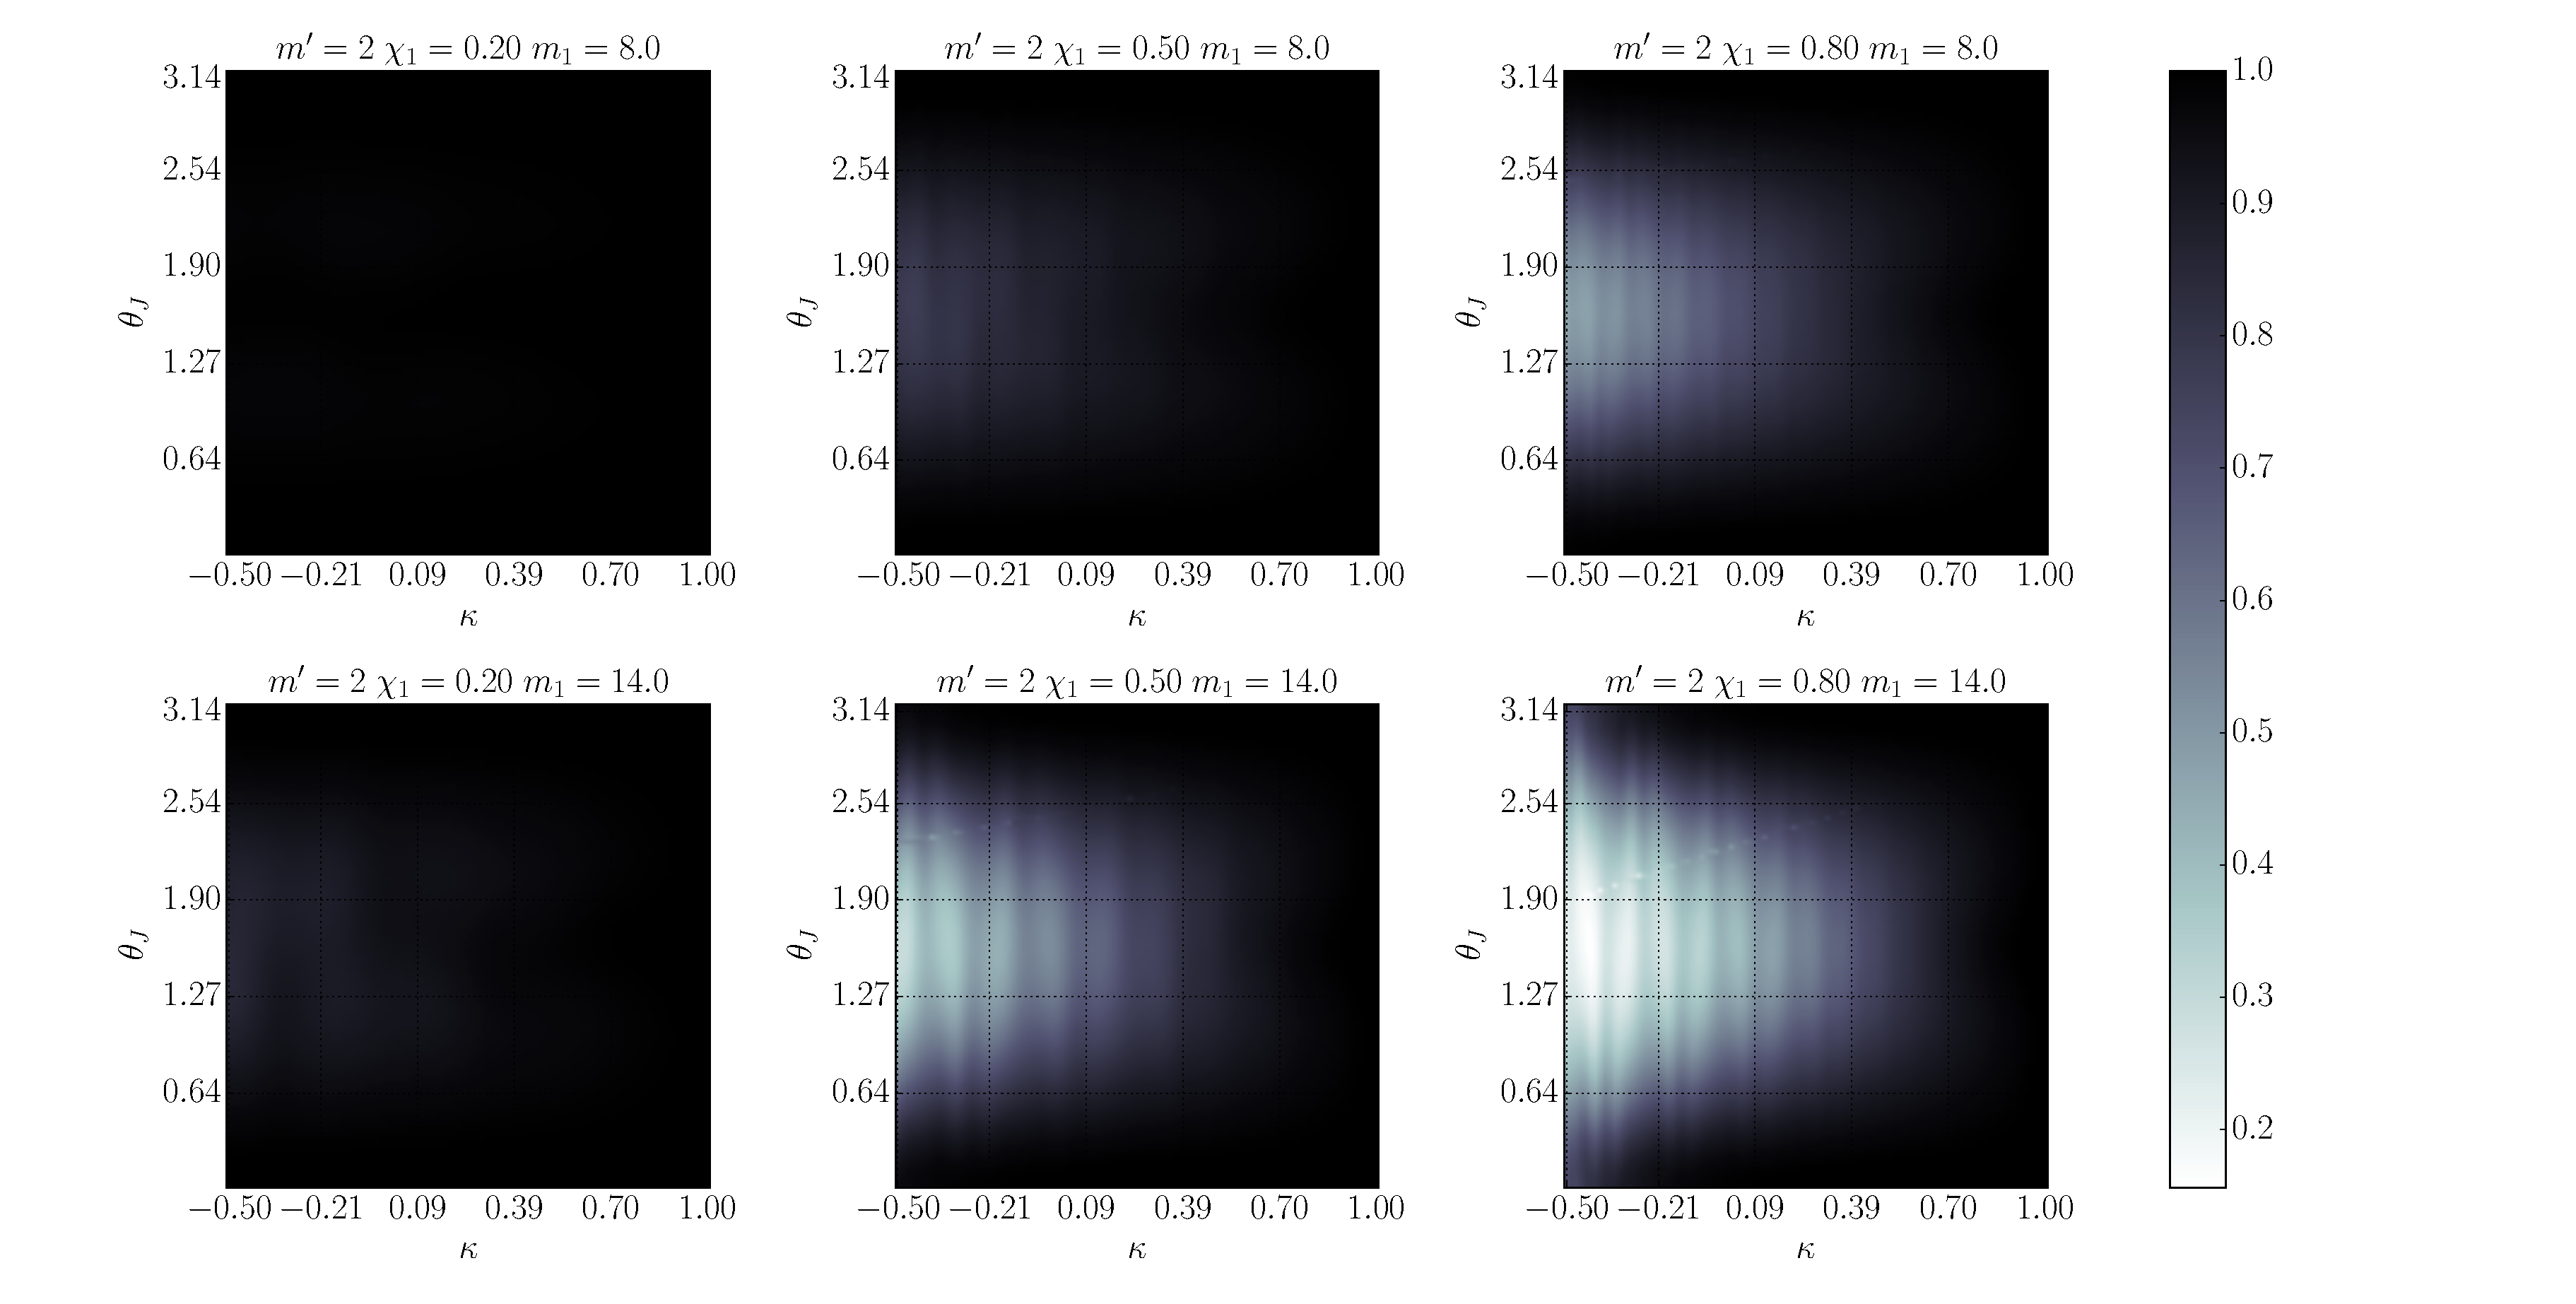
\includegraphics[width=\textwidth]{./images/OVLP_GRID_P2.pdf}
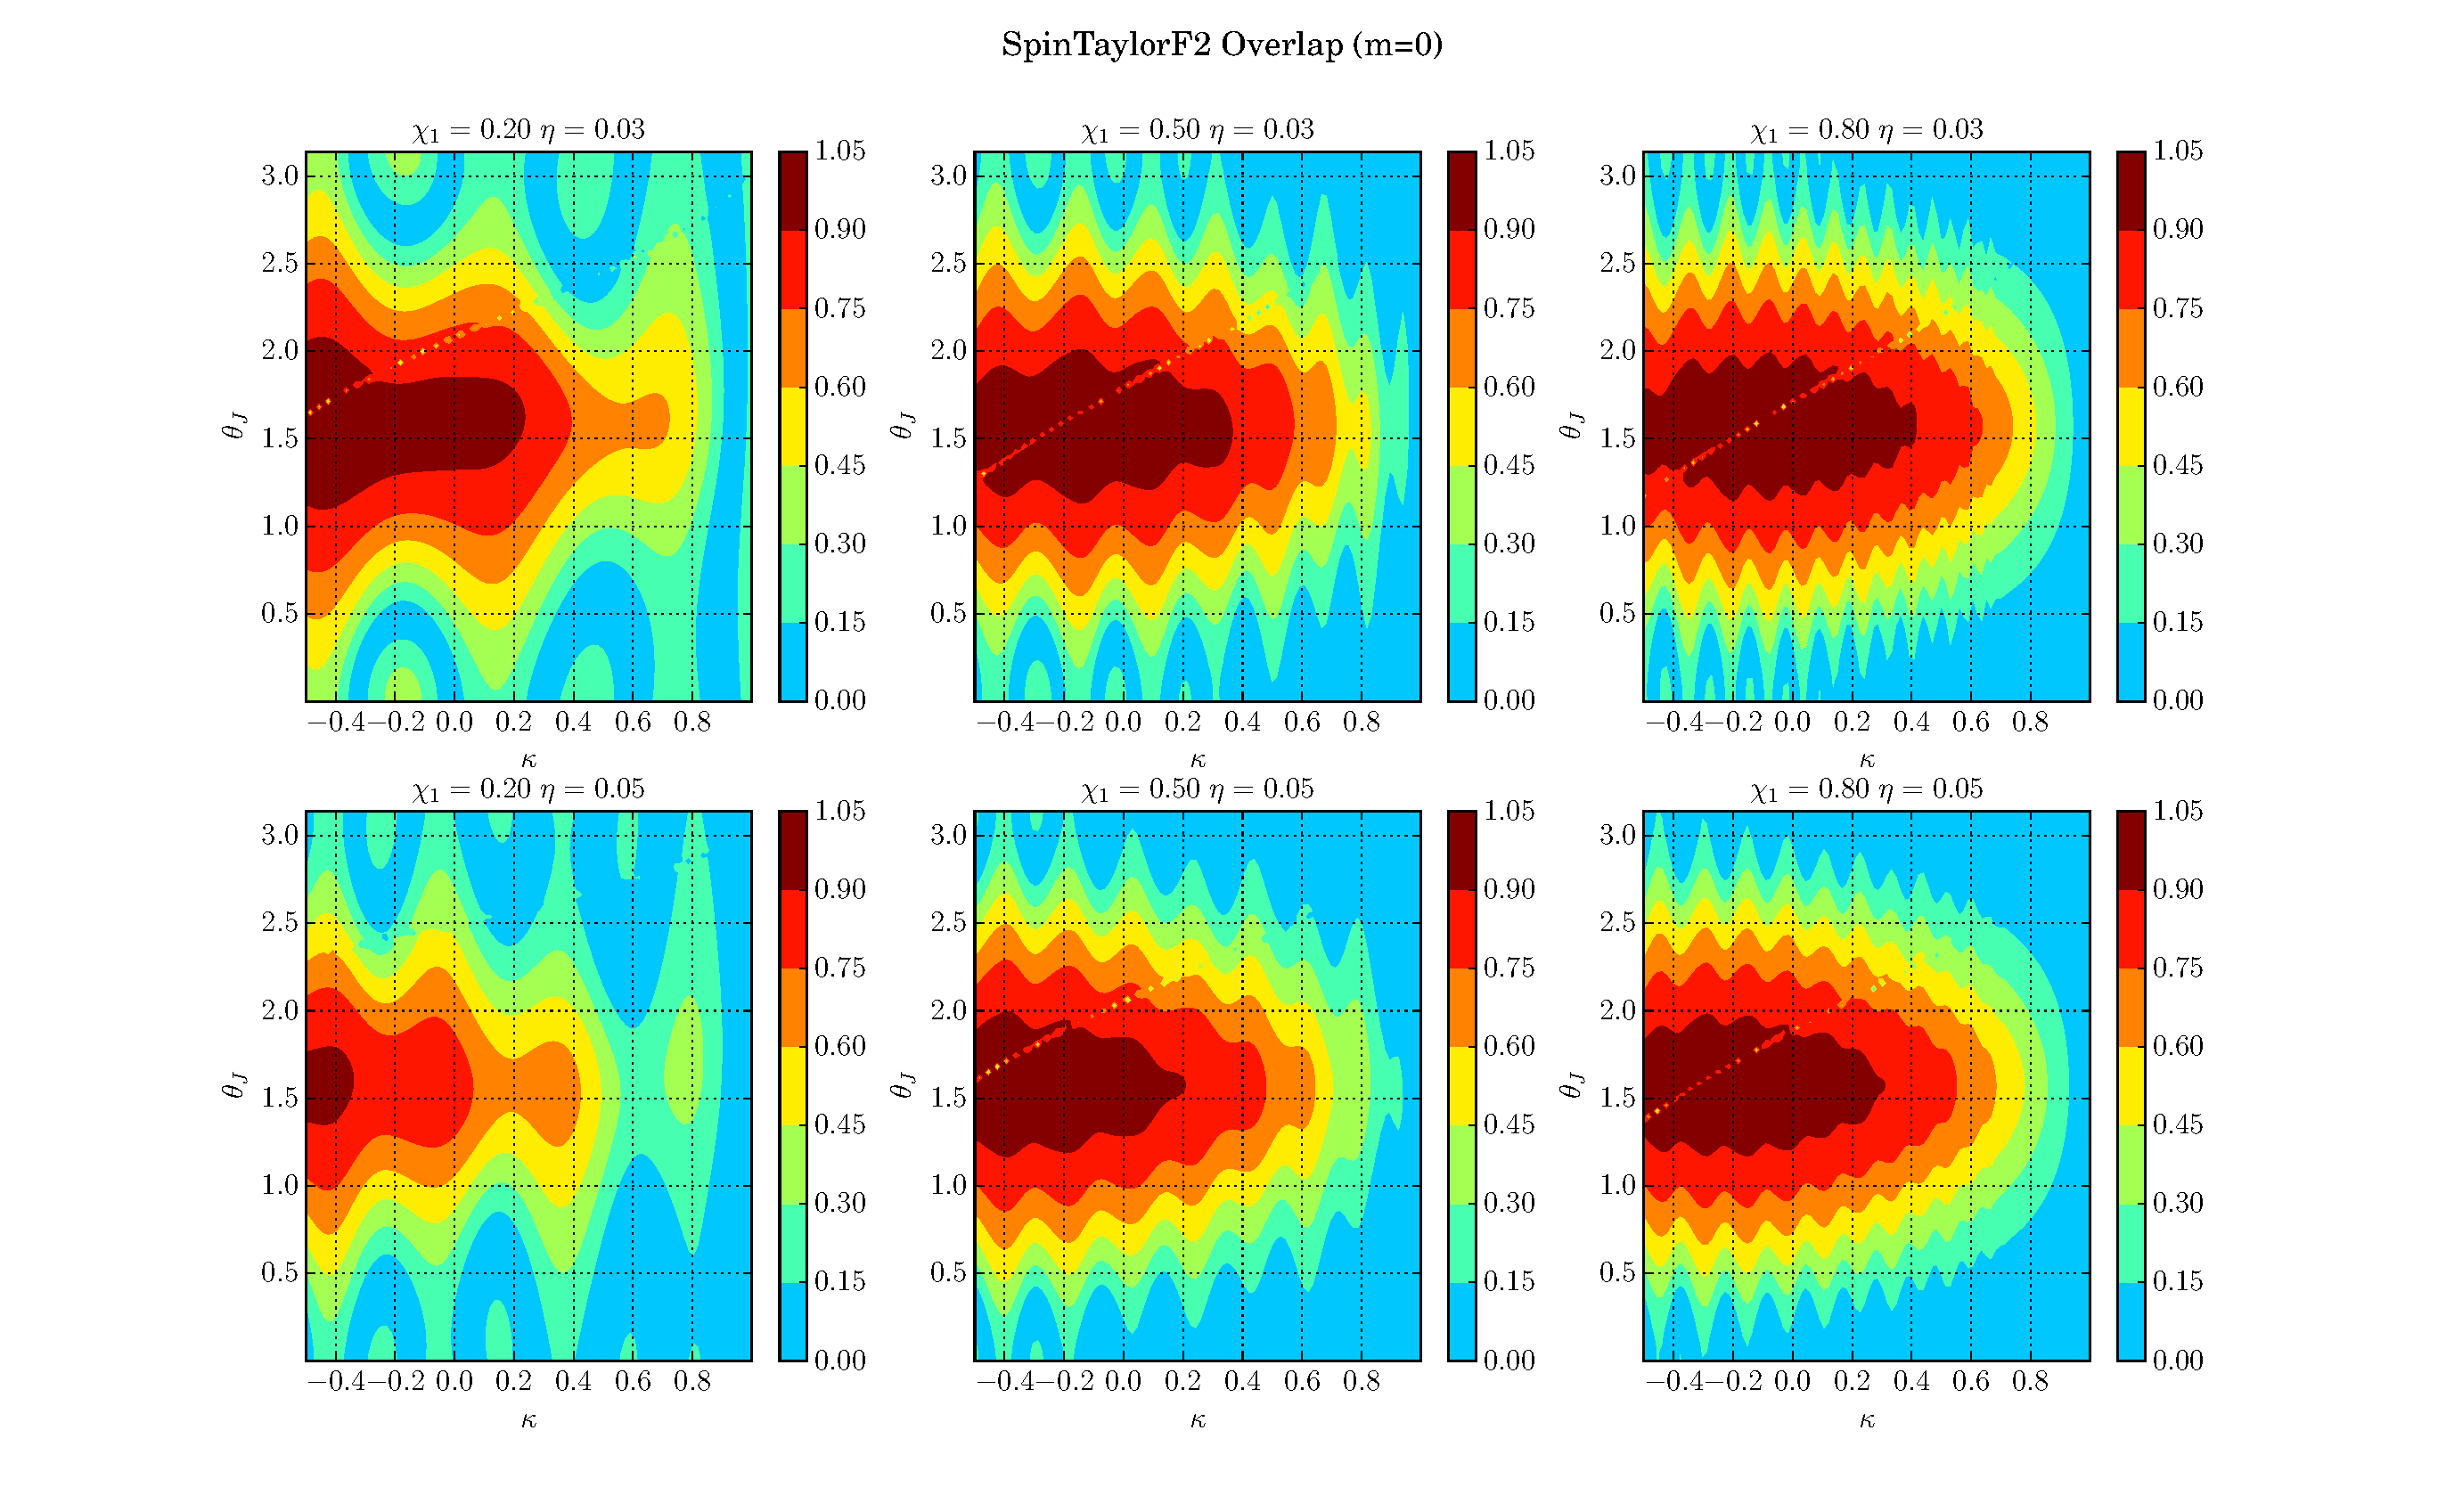
\includegraphics[width=\textwidth]{./images/OVLP_GRID_P0.pdf}
\caption{Overlaps plots} 
\centering 
\end{figure}

% \section{Future Work} 
% Our future work would be to investigate this claim by
% performing parameter estimation with the full SpinTaylorF2 waveform and compare
% the results when a specific sideband is used in the appropriate region of
% parameter space (precessing or non-precessing) which would help us figure out
% how faithfully do we recover parameters if we use sidebands instead of the full
% waveform in parameter estimation.








